\documentclass{article}
\usepackage[utf8]{inputenc}
\usepackage{float}
\usepackage{subcaption}

\title{LC 01 - Chimie et Couleur}
\author{Maria Ubero Gonzalez}
\date{Agrégation 2018-2019}

\usepackage{natbib}
\usepackage{graphicx}
\usepackage[a4paper, total={6in, 8in}]{geometry}

\begin{document}

\maketitle

\tableofcontents

\pagebreak

\section*{Introduction}
Les matières colorées sont connues et utilisées depuis la Préhistoire. Des fresques peintes avec des matières colorées minérales, telles que l'ocre ou le noir de charbon, ont été retrouvées dans des grottes ornées de peintures rupestres. Depuis la plus Haute Antiquité on sait extraire des matières colorées des végétaux, comme la garance, l'indigo ou le carthame; ou d'animaux, comme les kermès ou la cochenille des teintures. On appellait autrefois matières colorées organiques, les substances extraites des organismes vivants. Leur extraction était souvant longue et laborieuse, leur fixation sur support parfois imparfaite et leur coût de revient élevé.\smallskip

Dès le milieu du XIX ème siècle, les chimistes parviennent à synthétiser des espèces jusqu'à alors extraites de la nature. Les matières colorées naturelles sont alors progressivement remplacées par des produits de synthèse. Le terme organique change alors de définition. Une espèce organique naturelle ou de synthèse contient essentiellement les éléments carbone et hydrogène. Aujord'hui, une matière colorée peut être organique ou inorganique, naturelle ou synthétique.\medskip

\textit{Les peintures rupestres de la grotte de Lascaux laissent apparaître différentes couleurs : si le rouge et le noir sont
les deux couleurs les plus fréquemment utilisées, on trouve aussi, quoique plus rarement, le jaune, le brun, le
blanc. Le noir est du charbon minéral, mais le charbon de bois ou d’os était aussi employé ainsi que l’oxyde de
manganèse. Le rouge provient d’un oxyde de fer, l’hématite, qui est abondant dans les sols naturels. Toute la
gamme de couleurs allant du jaune au rouge est probablement issue des ocres qui contiennent des oxydes de fer.}

\begin{figure}[H]
\centering
\begin{subfigure}{.5\textwidth}
  \centering
  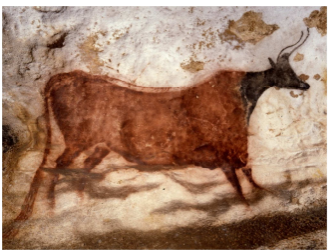
\includegraphics[width=.7\linewidth]{peinture.png}
  \caption{Vache rouge à tête noire }
  \label{fig:sub1}
\end{subfigure}%
\begin{subfigure}{.5\textwidth}
  \centering
  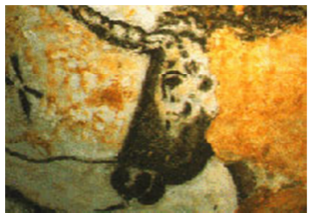
\includegraphics[width=.75\linewidth]{peinture2.png}
  \caption{Auroch de la salle des taureaux}
  \label{fig:sub2}
\end{subfigure}
\caption{Peintures rupestres de la grotte de Lascaux }
\label{fig:test}
\end{figure}

\section{Pourquoi voit-on de la couleur?}

Selon leur nature, les objets interagissent différemment avec la lumière.
\begin{itemize}
    \item La diffusion est le phénomène par lequel un objet éclairé renvoie dans toutes les directions la lumière incidente.
    \item La transmission est le phénomène par lequel un objet transparent est traversé par une partie de la lumière incidente. (c'est ce que notre oeil voit)
    \item L'absorption est le phénomène par lequel un objet éclairé absorbe une partie de la lumière incidente.
\end{itemize}

La transformation de la lumière blanche en lumière colorée, par réflexion sur un corps, par transmission ou diffusion, résulte de l'absorption sélective d'énergie par certains groupes d'atomes.\medskip

\textbf{Comment obtenir des couleurs?} \medskip

L'oeil perçoit les objets grâce aux images qui se forment sur la rétine. Il perçoit les couleurs grâce aux deux types de cellules photoréceptrices qu'il possède: les bâtonnets, très sensibles à l'intensité lumineuse mais pas aux couleurs, et les cônes qui détectent les lumières colorées.
Il existe trois types de cônes, chacun d'eux étant principalement sensible à une des couleurs primaires : rouge, vert ou bleu.\medskip

En \textbf{synyhèse soustractive}, la combinaison des couleurs cyan, magenta et jaune est suffisante pour recréer quasiment toutes les couleurs. On réalise une synthèse soustractive lorsqu'on supprime une partie du spectre d'une lumière afin d'obtenir une couleur différente. \medskip

Quand on superpose plusieurs lumières colorées, le cerveau en perçoit une nouvelle. C'est la \textbf{synthèse additive} des couleurs. On obtient une infinité de couleurs en combinant les tons de couleur rouge, verte et bleue.

\begin{center}
    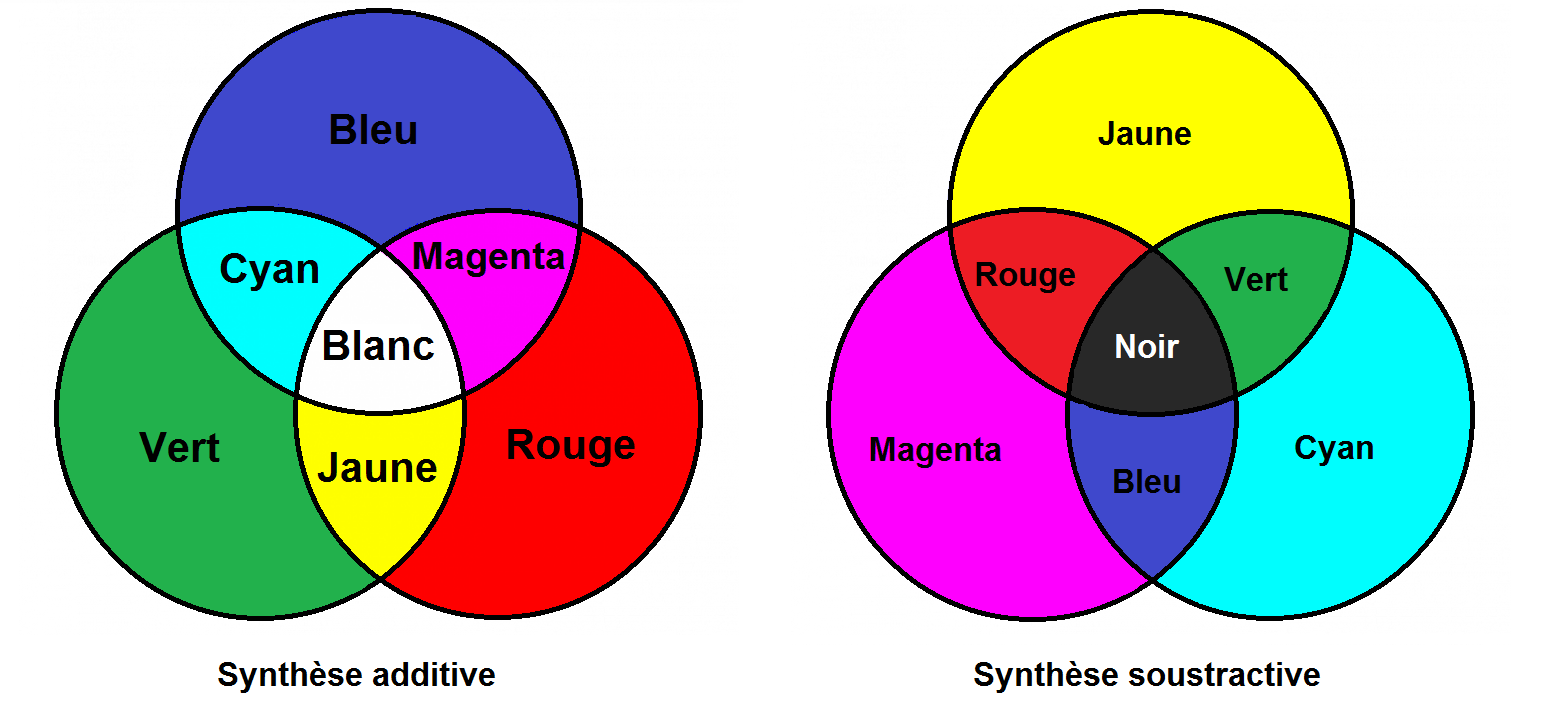
\includegraphics[scale=0.35]{Synthesesoustraddit.jpg}
\end{center}



\section{Origines chimiques des couleurs}
\subsection{Pigments et colorants}
Les molécules de la matière colorée sont classées en deux catégories suivant leur solubilité dans le milieu coloré; les colorants et les pigments.
\begin{itemize}
    \item Les colorants sont des espèces solubles dans le milieu qu'ils colorent. Ils sont présentes dans l'alimentation et en particulier les boissons et les bonbons mais ils sont aussi utilisés pour teindre les vêtements et dans les encres. 
    
    \item Toute comme un colorant, les pigments modiffient la couleur du milieu qui les reçoit mais à différence de ce dernier ils se présentent sous forme de poudre insoluble. Il est donc important de choisir un milieu qui puisse maintenir les pigments sans qu'il n'y ait décantation. Un tel milieu est appelé un ”liant” et peut par exemple être constitué d’huile. On peut retrouver des pigments dans des produits cosmétiques mais ils sont surtout présents dans les peintures.
\end{itemize}

\subsection{Synthèse et extraction}
Les pigments et les colorants peuvent être extraits d'une substance naturelle ou être synthétisés. Par exemple, l'indigo peut être extrait d'une plante, l'indigotier, ou synthétisé à partir de produits chimiques, ce qui permet de reduire sont prix de revient.\medskip

\textit{\textbf{MANIP. Synthèse de l'Indigo.}\\
Fait dans \textbf{Chime des couleurs et des odeurs}\\	
 \textbf{Réalisation (on divise tout par 2):} Dans un bécher dissoudre 1g de 2-nitrobenzaldéhyde dans 20 mL d'acétone et diluer la solution avec 35 mL d'eau. Agiter la solution en ajoutant 5 mL de soude 2 $mol.L^{-1}$. La couleur de la solution passe rapidement au jaune clair puis devient plus foncée et en quelques secondes un precipité d'indigo apparaît. Continuer d'agiter pendant 5 min puis essorer sous vide le precipité bleu-violet. Laver le solide à l'eau jusqu'à ce que les eaux de lavage soient incolores, puis à l'éthanol. Sécher le solide sous vide 5 à 10 min puis à l'étuve (100-120 degrées) 30 à 40 min.}OJO MIRAR COMO HACER EL RENDIMIENTO.\medskip

\textit{\textbf{MANIP. Utilisation de l'indigo en teinture. Réalisation :} Dans un erlenmeyer, dissoudre 0,5g de dithionite de sodium dans 40 mL d'eau chaude avec une pastille de soude. Ajouter 0,1g d'indigo et boucher l'erlenmeyer. Agiter la solution pendant quelques minutes jusqu'à ce que l'indigo soit dissous. La solution de la forme leuco a une teinte verte. Ajouter plus de dithionite de sodium si l'indigo n'est pas entièrement dissous. Immerger un échantillon de tissu dans la solution à l'aide d'un agitateur en verre. Reboucher l'erlenmeyer et agiter la solution. Après environ 30 secondes, retirer l'échantillon, le laver sous le robinet, le presser entre deux feuilles de papier essuie-tout, le laisser à l'air libre pour le sécher et pour permettre l'oxydation de la forme leuco par l'oxygène de l'air.}\medskip

Dire que l'indigo est très utilisé dans l'industrie textile, tissus...\medskip

\textit{\textbf{MANIP. Extraction colorants de la tomate.} Pas assez de temps...}

\subsection{Structure des molécules colorées}
Depuis la préhistoire, l'Homme a cherché des matières colorées qu'il pouvait utiliser. Il les a extrait des plantes ou des animaux. Ces substances ayant pour origine des organismes vivants sont qualifiées d'organiques.

\subsubsection{Les molécules organiques}
Historiquement une molécule organique est une molécule provenant d’un organisme vivant (animal ou végétal). Au XIXème siècle, les chimistes ont commencé à fabriquer des molécules identiques aux molécules organiques par synthèse en laboratoire. Aujourd’hui, on définit les molécules organiques comme molécules constituées essentiellement de l’élément carbone C et l’élément hydrogène H. \medskip

Une molécule organique est formée d’un enchaînement plus ou moins long d’atomes de carbone qui constituent le squelette carbone de la molécule. Ceux-ci sont principalement liés à des atomes d’hydrogène. Des groupes contenant d’autres éléments chimiques (oxygène, soufre, azote, chlore, fluor, etc...) peuvent être liés à ce squelette : on les nomme ”groupes
caractéristiques”. \medskip
 
 Exemple: la formule brute de l'indigo est $C_{16}H_{10}N_{2}O_{2}$
 
 \subsubsection{La représentation topologique des molécules}
La formule topologique est une représentation simplifiée des molécules organiques dans laquelle les atomes de carbone et les atomes d’hydrogène auxquels ils sont liés ne sont pas représentés.

\begin{itemize}
    \item Les liaisons carbone-carbone sont représentées par des segments
    \item Les doubles liaisons sont représentées par des doubles segments
    \item Seuls les atomes d’hydrogène portés par d’autres atomes que les atomes de carbone(hétéroatomes) sont représentés, les atomes de carbone en portant autant que nécessaire pour établir au total 4 liaisons covalentes.
\end{itemize}

\begin{figure}[H]
    \centering
    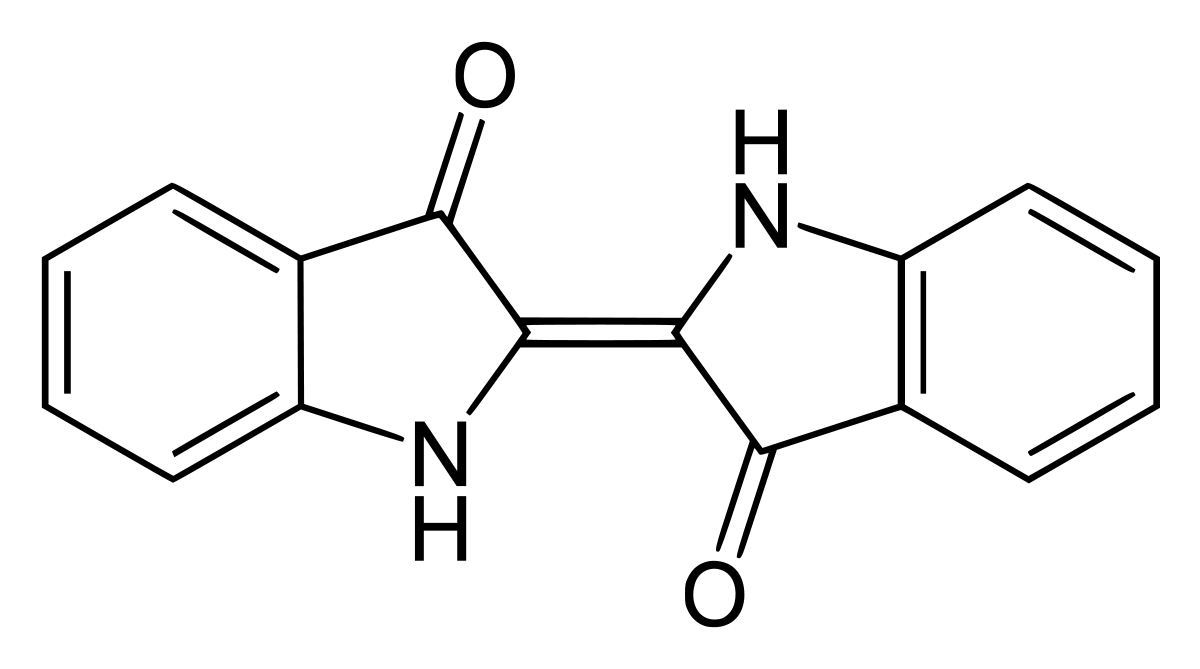
\includegraphics[width =6cm]{Indigomolecule.jpg}
    \caption{Indigo}
    \label{fig:my_label}
\end{figure}


\subsubsection{D'où vient la couleur?}

Les liaisons entre atomes sont assurées par des doublets d'électrons. L'interaction de la lumière avec la matière dépend de l'énergie des électrons des molécules et plus particulièrement de ceux des doubles liaisons $C=C, C=O,$ etc. \medskip

D'une manière générale:

\begin{itemize}
    \item Les molécules colorées présentent une alternance régulière de doubles liaisons et de simples liaisons : on dit que les doubles liaisons sont conjuguées ou en position conjuguée.
    \item Les molécules colorées absorbent certaines longueurs d'onde du domaine visible. La couleur perçue correspond à la couleur complémentaire des radiations absorbées.
    \item La longueur d'onde de la lumière observée augmente lorsque le nombre de doubles liaisons conjuguées augmente. En dessous de 7 doubles liaisons conjuguées, l’absorption se fait dans le domaine des ultraviolets ce qui ne donne pas de coloration perceptible pour les humains.
\end{itemize}

\begin{figure}
    \centering
    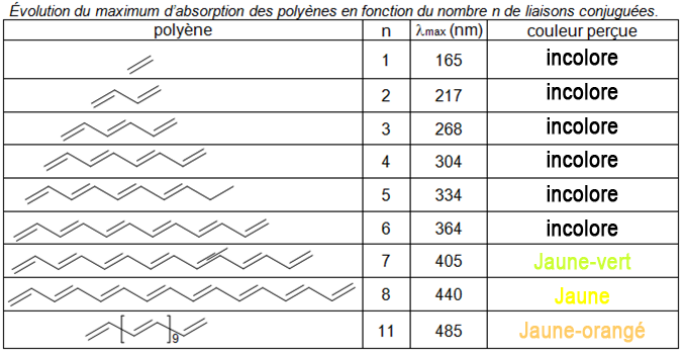
\includegraphics[scale=0.5]{Longonde.jpg}
    \caption{Liaisons conjuguées}
    \label{fig:my_label}
\end{figure}

La transformation de la lumière blanche en lumière colorée, par réflexion sur un corps, par transmission ou diffusion, résulte de l'absorption sélective d'énergie par certains groupes d'atomes appelés \textbf{chromophores}:\medskip

$-C=C-C=C-$\qquad $-C=N-$\qquad $-N=N-$\qquad $-C=C-C=O$
\medskip

Ils disposent d'orbitales vides ou incomplètes à des niveaux d'énergie peu éloignés de ceux des orbitales remplies, de sorte qu'ils absorbent la lumière visible d'énergie correspondant aux transitions possibles entre ces niveaux.\medskip

La présence de substituants peut modifier la longueur d'onde d'absorption. Le déplacement de l'absorption vers les plus grandes longueurs d'onde dans le doamine visible, est dû notamment à la présence de certains groupes \textbf{auxochromes} couplés aux groupes chromophhores. Parmi ces substituants, on peut citer : \medskip

$-NH_2$\qquad $-OH$\qquad $-O-CH_3$\qquad $-Br$
\medskip

En présence des auxochromes et ou de cycles présentant des doubles liaisons conjuguées, une molécule possédant un système conjugué de moins de 7 doubles liaisons peut colorer un matériau. Elle peut aussi provoquer un accroissement de l'intensité de la couleur.

\section{Influence des paramètres externes}

Certains paramètres extérieurs peuvent influencer la couleur d'un matériau organique:

\subsection{Influence du pH du milieu}
En changeant la valeur du pH de la solution dans laquelle se trouve une molécule organique, on peut modifier cette molécule. Il peut alors y avoir changement de la couleur de la solution. C'est le cas des espèces acido-basiques dont l'acide et la base ont des couleurs distinctes. Dans ce cas, suivant la valeur du pH, la forme acide ou basique est majoritaire et impose sa couleur. Le chou rouge contient des anthocyanes qui, suivant le pH, adoptent l’une de leurs quatre formes (cation flavylium (rouge), base quinionique (bleu-mauve), base carbinol (incolore) et chalcone (jaune clair)). La forme majoritaire impose sa couleur ; la large gamme de couleur est due à la grande variété d’espèces
colorées du chou rouge.\medskip

\textit{\textbf{MANIP. Extraction des colorants du chou rouge.}\\
\textbf{Le maréchal} Tome 1 chimie générale p147.\\
 \textbf{Réalisation:} Extraire le jus du choux rouge. Préparer 5 solutions de pH = 2, 5, 7, 9 et 12. Un même volume de bouillon de chou rouge est versé dans chacun des tubes à essai de l’échelle de pH : l’échelle de teinte observée s’étend du rouge (pH=2) au jaune(pH=12) en passant par le bleu(pH=7). Le choux rouge contient des colorants (les anthocyanes) qui ont la propriété de changer de couleur en fonction du pH.} \medskip

\textit{\textbf{MANIP. Bleu de bromothymol. Réalisation:} 3 solutions $HCl,\; c=0,1 mol/L, NaOH,\; c=0,1 mol/L$ et de l'eau distillée. Parler de la différence de structure de l'indicateur coloré en fonction de la couleur.}\medskip

\begin{figure}[H]
    \centering
    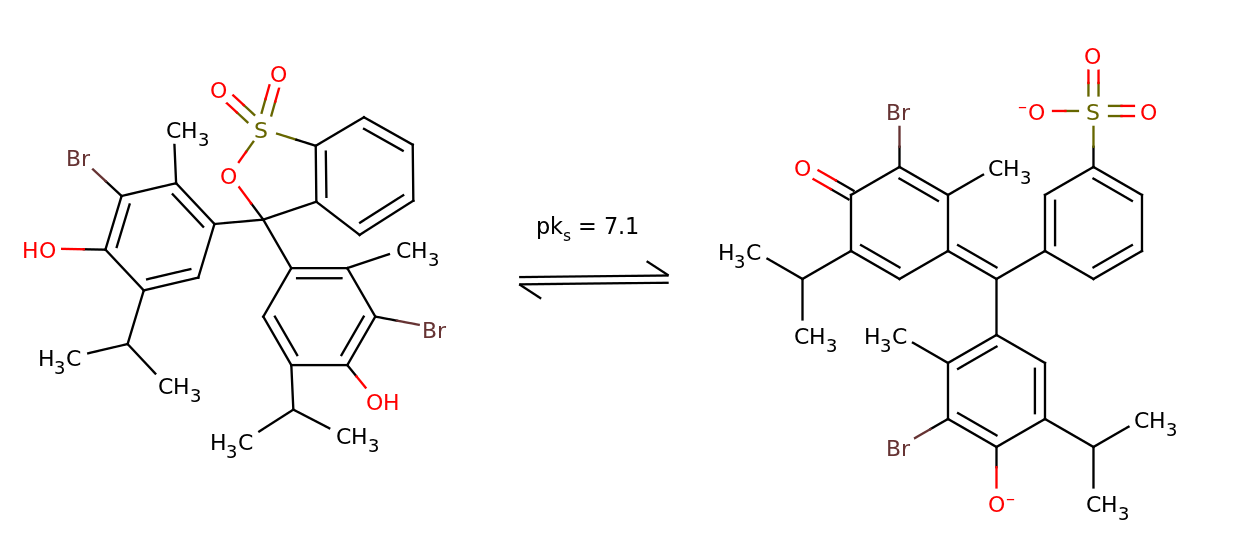
\includegraphics[width=10cm]{Bleu_de_bromothymol_forme_acide_basique.png}
    \caption{Bleu de bromothymol}
    \label{fig:my_label}
\end{figure}

Ces changements de couleur pour des solutions de pH différent sont largement utilisés pour détecter l’équivalence lors d’un dosage pH-métrique. Pour ce faire, on utilise des indicateurs colorés, c’est-à-dire des espèces colorées changeant de couleur suivant le pH de l’environnement. Le domaine de pH sur lequel ces espèces changent de couleur est prénommé zone de virage. Lors d’un dosage pH-métrique, la zone de virage de l’indicateur coloré doit se trouver au milieu du saut de pH comme illustré par la Figure 3. De cette manière, le changement de couleur aura lieu à l’équivalence.\medskip

GRAPHIQUE

\subsection{Influence du solvant}
Certaines espèces chimiques ont des couleurs différentes selon le solvant dans lequel elles sont dissoutes.\medskip

\textit{\textbf{MANIP Influence du solvant dans la coloration.} Le diiode $I_2$ adopte une coloration différente dans l’éthanol, l’eau, le cyclohexane et l’acétone. Le diiode est un composé apolaire, de couleur violette. Dans le cyclohexane, lui-même apolaire, il garde sa couleur violette. Par contre, le diiode intéragit avec les solvants polaires en délocalisant ses électrons . Il a alors une structure plus proche de ${I_3}^{-}$, qui est brun.\textbf{Réalisation:} Dans quatre tubes à essais, introduire, à l'aide d'une spatule, deux cristaux de diiode $I_2$. Verser respectivement 2ml d'eau, 2ml d'éthanol, 2ml de cyclohexane et 2 ml d'acétone. Boucher les tubes et agiter. Observer dans chaque cas la couleur de la solution. Dans l'eau (solvant polaire) jaune très pale, cyclohexane (solvant apolaire) rose, éthanol (solvant polaire) ??, acétone (solvant polaire) ??}

\subsection{Influence d'autres facteurs}
Certains matériaux changent de couleur sous l'effet d'un paramètre extérieur. Ainsi une radiation lumineuse modifie la couleur des espèces \textbf{photochromes} utilisées dans les verres pour les lunettes. Pour les matériaux \textbf{thermochromes} c'est une variation de température qui modifie la couleur de la matière. 
Donner des exemples: chauffage de l'ocre...

\section{Caractérisation de la couleur d'une solution}
Une solution se comporte comme un filtre coloré, lorqu'elle est traversée par une lumière blanche, elle atténue l'intensité de certaines radiations qui sont dites absorbées.
\subsection{Absorbance}
L'absorbance est une grandeur physique qui traduit la capacité d'un milieu a absorber un rayonnement. Elle est définie comme:

\begin{equation}
    A = -\log{\frac{I}{I_0}}
\end{equation}

avec $I_0$ l’intensité lumineuse de référence et I l’intensité transmise par la solution. Cette mesure s’effectue avec un spectrophotomètre. Le principe est le suivant : une source lumineuse de longueur d’onde ajustable éclaire une cuve contenant la solution à étudier. Un photodétecteur mesure l’intensité transmise par la solution. Afin de s’affranchir de l’absorption du solvant, un étalonnage avec du solvant pur est nécessaire et détermine $I_0$.\medskip

Pour une longueur d'onde donnée: Une valeur $A=0$ signifie que la solution est complètement transparente : la radiation incidente n’est pas du tout absorbée. Une valeur $A=1$ signifie que 90 $\%$ de l’énergie lumineuse de la radiation incidente est absorbée. \medskip

Le spectre d'absorption d'une solution est le graphique représentant son absorbance en fonction de la longueur d’onde.\medskip

\textit{\textbf{MANIP Spectre d'absorption du Schtroumpf mesuré avec le spectrophotomètre.} Vérifier que le pic maximal d'absorption est dans le rouge $(\lambda= 640 nm)$, comparer le spectre d'absorption obtenu avec le spectre du colorant bleu patenté V (additif E131). \textbf{Réalisation:} Seule la partie bleue du bonbon est à prélever afin de répondre à la problématique. Il faut donc ôter le chapeau du bonbon. Dissoudre dans 30-40 ml d'eau, il convient de chauffer la solution à l’aide d’un agitateur magnétique muni d’une plaque chauffante (la durée indicative de chauffage est de 5 min environ). A l’aide d’un spectrophotomètre disposant d’un balayage automatique des longueurs d’ondes du visible, on trace la représentation graphique $A= f(\lambda)$. Comparation avec spectre du E131.}

\begin {figure}[H]
\centering
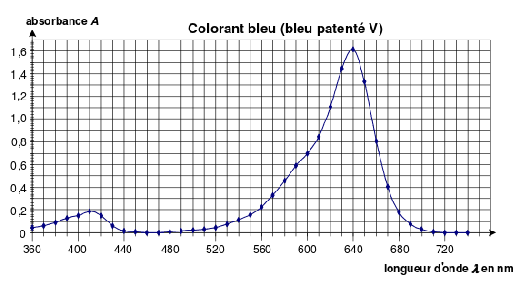
\includegraphics [width =13cm]{E131spectre.jpg}
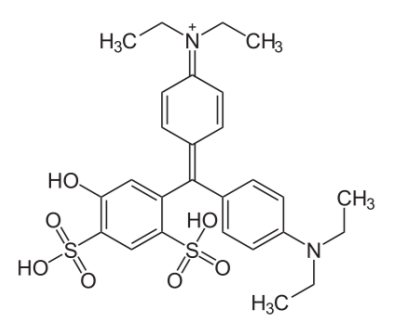
\includegraphics [width =5cm]{E131molecule.jpg}
\caption {Bleu patente V}
\end {figure}

\subsection{Loi de Beer Lambert}

L’absorbance $A_{\lambda}$ d'une solution dépend de la concentration molaire $C$ de l'espèce colorée et de la longueur $l$ de la cuve :

\begin{equation}
    A_{\lambda} = \sum_{i=1}^{n}\epsilon_{i\lambda}lc_i
\end{equation}

$\epsilon_{\lambda}$ appelé coefficient d'absorption molaire (en $L.mol^{-1}.cm^{-1}$), est une grandeur dépendant de la nature de l'espèce chimique et de la longueur d'onde $\lambda$, $c$ est la concentration de la solution (en $mol.L^{-1}$) l est l'épaisseur de la cuve (en $cm$).\medskip

\textbf{Domaine de validité:} Il ne doit pas y avoir de solides dans la solution, les solutions doivent être diluées (en général $c < 10^{-2}$).

\subsection{Application à un dosage}

\textit{Peut-on manger le contenu d'un paquet de Schtroumpfs sans risque de toxicité vis-à-vis du colorant?}\medskip

La loi de Beer Lambert permet de doser une espèce chimique colorée puisq'elle permet d'etablir la relation entre l’absorbance A et la concentration C de l’espèce étudiée en solution.\medskip

\textit{\textbf{MANIP. Dosage du colorant bleu patenté V dans les Schtroumpfs.} \textbf{Réalisation:} Faire une échelle de teinte à partir d'une solution de bleu patenté V à $1,0.10^{-5} mol.L^{-1}$. Tracer la droite d'étalonnage $A=f(c)$. En mesurant pour $\lambda_max = 640 nm$ l’absorbance d’un échantillon de la solution bleue de bonbon Schtroumpf, on détermine par construction graphique sa concentration molaire
volumique. La masse de bleu patenté V contenu dans un bonbon est $m = cVM$. Masse molaire $M=560 g.mol^{-1}$. Selon la DJA (Dose Journalière Admissible): 2,5 mg par kilogramme de masse corporelle. Pour une personne de 65 kg, calculer combien de mg par jour et finalement combien de bonbons par jour elle peut manger.}

\section{Conclusion}
La Nature et la chimie regorgent de couleurs variées, plus ou moins vives et qui ont souvent des intérêts particuliers (ex : les couleurs vives de certaines plantes servent à attirer les insectes et autres oiseaux pour favoriser la dispersion du pollen). Ces couleurs peuvent être caractérisées quantitativement par des mesures d’absorbance en ce qui concerne les solutions. Grâce à la loi de Beer-Lambert, il est ensuite possible d’estimer les concentrations en espèces colorées.
La couleur d’une espèce est due aux pigments ou aux colorants, qui peuvent être extraits ou synthétisés. Ce sont des molécules possédant de longues liaisons délocalisées absorbant une partie de la lumière. Nonobstant, la couleur dépend de divers paramètres comme le solvant utilisé, le pH du milieu ou même la température. La couleur d’une solution est donc une source précieuse d’indications sur la solution elle-même.
En appliquant des méthodes similaires en sortant du domaine visible, dans les infrarouges (IR) par exemple, on peut également obtenir des informations sur les molécules et leur structure en mesurant leur spectre d’absorption.

\section*{Questions que je me pose:}
\begin{itemize}
\item \textbf{Avantages et inconvénients des espèces naturelles et produits de synthèse?}
 Avantages : les colorants synthétiques permettent de produire en plus grande quantité avec des coûts très inférieurs aux colorants naturels. De plus, ils permettent de mettre en avant de nouvelles inventions et couleurs qui sont inventées dans ce même courant de révolution industrielle, comme le fluo, aux XIXème siècle.\medskip
 Inconvénients : contraintes des colorants synthétiques. Dans la législation, un colorant alimentaire est "une substance qui peut entrer dans la composition de certains aliments dans un but bien déterminé et selon des conditions définies par la loi ". Ceux-ci sont parfois considérés comme dangereux pour l'organisme. En effet, ce sont des substances étrangères à l'organisme qui n'ont jamais été testées chez les êtres humains. Si ils sont consommés en grande quantité, ils sont en majorité cancérigènes mais on ignore les conséquences sur l'organisme sur une longue durée. 

\end{itemize}
\section*{Questions}
L'indigo est il soluble dans l'eau ? Si non dans quoi est il soluble ? Sa couleur change t'elle selon le solvant ?\\

Dans la synthèse de l'indigo, la soude joue t-elle un rôle ?\\

Quelle est l'espèce formée par la cétone en milieu basique ?\\

Y a t'il une alternance de simples et de doubles liaisons dans l'indigo ? Si non pourquoi l'indigo est il si coloré ?\\
Parce que les doublets non liants de l'azote sont délocalisés à l'échelle de la molécule $\rightarrow$ molécule très conjuguée.\\

Hors du programme de 1ere : y a t'il d'autres molécules/atomes/ions colorés ?\\

Est ce l'absorbance qui caractérise la couleur ?\\
Non elle caractérise son intensité, il faut bien mettre an valeur le fait que c'est la longueur d'onde correspondant au max de A qui compte.\\

Pourquoi le bleu de patenté est il toxique ? Que risque t'on en en consommant trop ?\\



\section*{Remarques}
Pour l'indigo, lorsqu'on rince à l'éthanol : enlever l'eau d'abord pour pouvoir jeter l'éthanol à part.\\
Attention le logarithme n'est pas au programme de première.\\
Concernant la manip avec le BBT : il est naturellement donné en solution basique : si on veut voir sa couleur en milieu basique il faut donc le mettre dans une solution tampon à 7.\\
Le diiode n'est pas soluble dans l'eau : on le met donc avec de l'iodure $I^-$ afin d'avoir$I_3^{-}$ en solution.\\
Possibilité d'utiliser la phénolphtaléïne.\\
Possibilité de remplacer le diiode par du chou-rouge.\\
Indigo : si on obtient une forme protonée ou déprotonée, qui possède donc des propriétés acido-basiques, on pourra alors la solubiliser dans l'eau.\\
Le rouge para fonctionne bien aussi.\\
Parler de la notion de couleur spectrale.\\
Regarder livres : "la couleur dans tous ces états", et "lumière et luminescence". \\

\bibliographystyle{plain}
\bibliography{references}
\end{document}
